% CN 12.7 Exercises (p.447--449)

% ======================================================================
\begin{exercise}{1}
    Draw all trees that have six vertices (every tree on six vertices should be
    identical to one in your set, up to relabelling and redrawing).
\end{exercise}

\begin{exercise}{2}
    The \emph{diameter} of a graph is the length of the longest path in it.
    Prove that every tree of diameter $\ge3$ has a vertex $v$ such that
    \[
        2\le\deg(v)\le n-2,
    \]
    where $n$ is the number of vertices.
\end{exercise}

\begin{exercise}{3}
    If a tree has $k$ vertices of degree 3 and all other vertices are leaves, how
    many leaves does it have?
\end{exercise}

\begin{exercise}{4}
    \begin{enumerate}[label=(\alph*)]
        \item Prove that every tree with at least three vertices has a vertex of
              degree at least 2.
        \item Is there a number $N$ such that every tree with at least $N$
              vertices has a vertex of degree at least 3?
    \end{enumerate}
\end{exercise}

\begin{exercise}{5}
    Prove that a graph $G$ is a tree if and only if for every pair $u,v$ of
    vertices, there is a unique path between them in $G$.
\end{exercise}

\begin{exercise}{6}
    Give an upper bound on the average degree of a tree.
\end{exercise}

\begin{exercise}{7}
    How many spanning trees does the following graph have?
    \begin{center}
    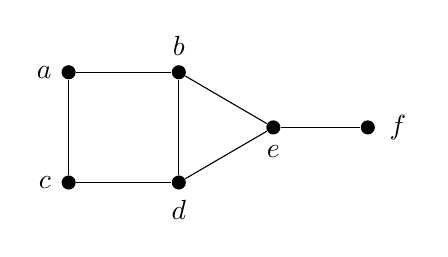
\begin{tikzpicture}[every node/.style={circle,fill,inner sep=1.8pt}]
        \node[label=left:$a$] (a) at (0,1.4) {};
        \node[label=above:$b$] (b) at (1.4,1.4) {};
        \node[label=left:$c$] (c) at (0,0) {};
        \node[label=below:$d$] (d) at (1.4,0) {};
        \node[label=below:$e$] (e) at (2.6,0.7) {};
        \node[label=right:$f$] (f) at (3.8,0.7) {};
        \draw (a)--(b)--(d)--(c)--(a);
        \draw (b)--(e)--(d);
        \draw (e)--(f);
    \end{tikzpicture}
    \end{center}
\end{exercise}

\begin{exercise}{8}
    Apply Kruskal's Greedy Algorithm to find a minimum weight spanning tree in the
    following weighted graph.
    \begin{center}
    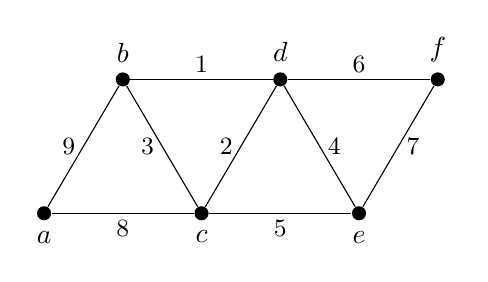
\begin{tikzpicture}[every node/.style={circle,fill,inner sep=1.8pt},
                        lab/.style={fill=none,draw=none,inner sep=1pt,font=\small}]
        \node[label=below:$a$] (a) at (0,0) {};
        \node[label=below:$c$] (c) at (2,0) {};
        \node[label=below:$e$] (e) at (4,0) {};
        \node[label=above:$b$] (b) at (1,1.7) {};
        \node[label=above:$d$] (d) at (3,1.7) {};
        \node[label=above:$f$] (f) at (5,1.7) {};
        \draw (b)--node[lab,above]{1}(d);
        \draw (d)--node[lab,above]{6}(f);
        \draw (a)--node[lab,left]{9}(b);
        \draw (b)--node[lab,left]{3}(c);
        \draw (c)--node[lab,left]{2}(d);
        \draw (d)--node[lab,right]{4}(e);
        \draw (e)--node[lab,right]{7}(f);
        \draw (a)--node[lab,below]{8}(c);
        \draw (c)--node[lab,below]{5}(e);
    \end{tikzpicture}
    \end{center}
\end{exercise}

\begin{exercise}{9}
    Prove that $K_{2,n}$ is planar for all $n$.
\end{exercise}

\begin{exercise}{10}
    Check that Euler's Theorem ($n-m+f=2$) holds for the following graphs:
    \begin{enumerate}[label=(\alph*)]
        \item the cycle $C_n$;
        \item the wheel graph $W_n$, obtained from $C_n$ (the ``rim'') by adding
              a new vertex (the ``hub'') adjacent (via ``spokes'') to every vertex
              of $C_n$;
        \item $K_4$;
        \item the cube $Q_3$ (Exercise 11.11);
        \item the octahedron;
        \item the dodecahedron;
        \item the icosahedron.
    \end{enumerate}
\end{exercise}

\begin{exercise}{11}
    \begin{enumerate}[label=(\alph*)]
        \item Give an upper bound on the average degree of a planar graph.
        \item Give an upper bound on the average degree of a planar graph with no
              triangles.
        \item Give an upper bound on the average degree of a bipartite planar
              graph.
    \end{enumerate}
\end{exercise}

\begin{exercise}{12}
    Prove that every planar graph has a vertex of degree $\le5$.
\end{exercise}

\begin{exercise}{13}
    Let $d\in\N$. A graph is \emph{$d$-regular} if every vertex has degree $d$.
    \begin{enumerate}[label=(\alph*)]
        \item Find the 3-regular planar graph with the fewest vertices.
        \item Find the 3-regular bipartite planar graph with the fewest vertices.
        \item Find the 3-regular nonplanar graph with the fewest vertices.
        \item Describe an infinite family of connected 4-regular planar graphs.
        \item What is the minimum number of vertices of a 5-regular planar graph?
              Can you find such a graph?
        \item Does a 6-regular planar graph exist? Justify your answer.
    \end{enumerate}
\end{exercise}
